% !Mode:: "TeX:UTF-8"
% !TEX TS-program = xelatex
\documentclass[UTF8]{report}
% \documentclass[UTF8]{report}

\usepackage[zihao=-4,heading=true]{ctex}
\usepackage{geometry}
\geometry{left=2.0cm, right=2.0cm, top=2.0cm, bottom=2.0cm}
\usepackage[colorlinks=true]{hyperref}
\usepackage{graphicx} % used for add figure to this report
\graphicspath{{img/}}
\usepackage{listings}
\usepackage{xcolor}
\usepackage{booktabs}
\usepackage[toc]{multitoc}
\usepackage{graphics}
\usepackage{subfig}
\usepackage{fancyhdr}
\usepackage{enumerate}
\usepackage[section]{placeins}


	\lstdefinestyle{customcpp}{
		numbers=left,
		numberstyle=\tiny,
		belowcaptionskip=1\baselineskip,
		breaklines=true,
		xleftmargin=\parindent,
		language=C++,
		showstringspaces=false,
		basicstyle=\footnotesize\ttfamily,
		keywordstyle=\bfseries\color{green!40!black},
		commentstyle=\itshape\color{purple!40!black},
		identifierstyle=\color{blue},
		stringstyle=\color{orange},
	}
	
	\lstdefinestyle{customjava} {
	language=Java,
	backgroundcolor=\color{lightgray},
	breaklines=true,
	% numbers=left,
	% numberstyle=\tiny,
	basicstyle=\ttfamily,
	keywordstyle=\bfseries\color{green!40!black},
	commentstyle=\itshape\color{purple!40!black},
	identifierstyle=\color{blue},
	stringstyle=\color{orange},
}	

\lstdefinestyle{myxml} {
    backgroundcolor=\color{lightgray},
	language=XML,
	breaklines=true,
    % numbers=left,
	% numberstyle=\tiny,
	basicstyle=\ttfamily,
	keywordstyle=\bfseries\color{green!40!black},
	commentstyle=\itshape\color{purple!40!black},
	identifierstyle=\color{blue},
	stringstyle=\color{orange},
}
\lstdefinestyle{mysh} {
    backgroundcolor=\color{lightgray},
	language=sh,
	breaklines=true,
    % numbers=left,
	% numberstyle=\tiny,
	basicstyle=\ttfamily,
	keywordstyle=\bfseries\color{green!40!red},
	commentstyle=\itshape\color{purple!40!black},
	identifierstyle=\color{blue},
	stringstyle=\color{orange},
}
\lstdefinestyle{mysql} {
    backgroundcolor=\color{lightgray},
	language=SQL,
	breaklines=true,
	basicstyle=\ttfamily,
	keywordstyle=\bfseries\color{green!40!red},
	commentstyle=\itshape\color{purple!40!black},
	identifierstyle=\color{blue},
	stringstyle=\color{orange},
}


\lstdefinestyle{normal} {
	language=sh,
	basicstyle=\ttfamily,
	breaklines=true,
	keywordstyle=\bfseries\color{green!40!red},
	commentstyle=\itshape\color{purple!40!black},
	identifierstyle=\color{blue},
	stringstyle=\color{orange},
}

\lstset{style=normal}

\ctexset {
part/pagestyle = empty,
chapter = {
    format = \raggedright,
    pagestyle = empty,
},
section = {
    name = {第,部分},
    number = \chinese{section},
},
subsection = {
    name = {第,节},
    number = \chinese{subsection},
}
}
\pagestyle{fancy}

\titleformat{\section}
            {\LARGE\bfseries\sffamily\color{RoyalBlue}}
            {
\includegraphics[height=2em]{hadoop/hadoop2.png} \thesection{}.}
            {1em}
            {\huge\scshape}


\begin{document}
Spark SQL的前身是Shark,Shark是伯克利实验室Spark生态环境的组件之一,它能运行在Spark引擎上,从而使得SQL查询的速度得到10-100倍的提升,但是,随着Spark的发展,由于Shark对于Hive的太多依赖(如采用Hive的语法解析器、查询优化器等等),制约了Spark的One Stack Rule Them All的既定方针,制约了Spark各个组件的相互集成,所以提出了SparkSQL项目。
SparkSQL抛弃了原有Shark的代码,汲取了Shark的一些优点,如内存列存储(In-MemoryColumnarStorage)、Hive兼容性等,重新开发了SparkSQL代码;由于摆脱了对Hive的依赖性,SparkSQL无论在数据兼容、性能优化、组件扩展方面都得到了极大的方便。
SQLContext具体的执行过程如下:
\begin{figure}[htbp]
    \centering
    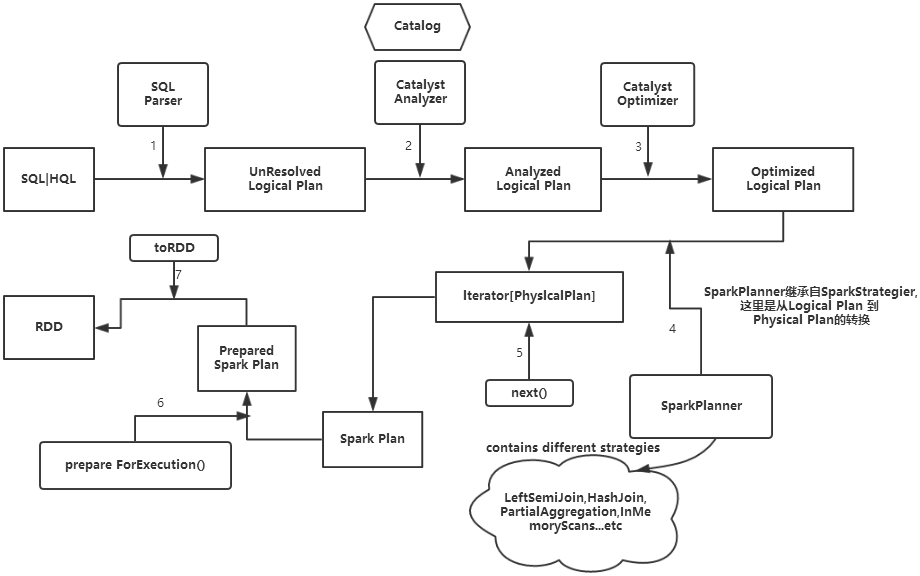
\includegraphics[width=\linewidth]{spark/spark-sql.png}
    \caption{Spark SQL执行流程}
    \label{fig:spark_sql}
\end{figure}

\begin{enumerate}[1)]
\item SQL | HQL语句经过SqlParse解析成UnresolvedLogicalPlan。
\item 使用analyzer结合数据字典(catalog)进行绑定,生成resolvedLogicalPlan,在这个过程中,Catalog提取出SchemRDD,并注册类似case class的对象,然后把表注册进内存中。
\item Analyzed Logical Plan经过Catalyst Optimizer优化器优化处理后,生成Optimized Logical Plan,该过程完成以后,以下的部分在Spark core中完成。
\item Optimized Logical Plan的结果交给SparkPlanner,然后SparkPlanner处理后交给PhysicalPlan,经过该过程后生成Spark Plan。
\item 使用SparkPlan将LogicalPlan转换成PhysicalPlan。
\item 使用prepareForExecution()将PhysicalPlan转换成可执行物理计划。
\item 使用execute()执行可执行物理计划。
\item 生成DataFrame。
\end{enumerate}
在整个运行过程中涉及到多个SparkSQL的组件,如SqlParse、analyzer、optimizer、SparkPlan等等。


\end{document}